

\input{"C:/Users/spileggi/Google Drive/STAT 330/Lectures/SlideStyle.tex"}



\title[Lecture 14]{Retain/Sum, PROC SORT, and First./Last.}
\author[Pileggi]{Shannon Pileggi}

\institute[STAT 330]{STAT 330}

\date{}


\begin{document}

\begin{frame}
\titlepage
\end{frame}

\begin{frame}
\frametitle{OUTLINE\qquad\qquad\qquad} \tableofcontents[hideallsubsections]
\end{frame}

%===========================================================================================================================
\section[Retain/Sum]{Retain/Sum}
%===========================================================================================================================
\subsection{}


\begin{frame}
\ft{RETAIN statement}
\bi
\item SAS DATA steps execute \emph{line by line} and \emph{observation by observation}.
\item In doing so, SAS makes use of the Program Data Vector (PDV).
\item The PDV erases all entries each time it cycles through the observations.
\item \ttt{RETAIN} allows you to keep the value of a variable in the PDV.
\item This allows you to carry values forward to a new observation.
\ei
\end{frame}

\begin{frame}
\ft{Examples of \ttt{RETAIN}}
\bi
\item \fbox{\ttt{RETAIN month1 - month5;}}
\item[] retains the values of 5 variables (\ttt{month1} through \ttt{month5}), all initial values set to missing
\item \fbox{\ttt{RETAIN month1 - month5 (10 20 30 40 50);}}
\item[] retains the values of 5 variables (\ttt{month1} through \ttt{month5}), initial values set as 10, 20, 30, 40, and 50 respectively
\item \fbox{\ttt{RETAIN month1 - month5 1 year 0 a b c "XYZ";}}
\item[] retains the values of nine variables and sets their initial values
\bi
\item initial values of \ttt{month1} through \ttt{month5} are set to 1
\item initial value of  \ttt{year} is set to 0
\item the initial values of \ttt{a}, \ttt{b}, and \ttt{c} are set to the character value `\ttt{XYZ}'.
\ei
\ei
\end{frame}

\begin{frame}[fragile]
\ft{The data}
\bmp{1.0\textwidth}
\footnotesize
\begin{code}{.0}
DATA kids;
INPUT famid name $ birth age wt sex $ ;
DATALINES;
1 beth 1  9  75  f
. bob  2  6  45  m
. barb 3  3  20  f
2 andy 1  8  80  m
. al   2  6  50  m
. ann  3  2  25  f
3 pete 1  6  55  m
. pam  2  4  37  f
. phil 3  2  33  m
;
RUN;
\end{code}
\emp
\end{frame}

\begin{frame}[fragile]
\ft{Example 1 - Fix Family ID}
\bmp{0.7\textwidth}
\footnotesize
\begin{code}{.0}
DATA kids2 ;

   SET kids ;
   
   IF famid NE . THEN newid = famid ;
   
   RETAIN newid ;
   
   famid = newid ;
   
   DROP newid ;

RUN ;
\end{code}
\emp
%\bmp{0.05\textwidth} \hspace{1in} \emp
%\bmp{0.25\textwidth}
%\ttt{RETAIN} \textbf{only} works on \emph{newly} created variables.  \ttt{RETAIN} does not work on variables that already exist in the data set.
%\emp


\end{frame}



\begin{frame}
\ft{\ttt{SUM} statement}
\bi
\item A \ttt{SUM} statement looks like
\item[] \fbox{\emph{variable} \ttt{+} \emph{expression}\ttt{;}}
\item[] no equal sign needed
\item used to \emph{cumulatively} add the value of an expression to a variable
\item \ttt{SUM} is a special case of \ttt{RETAIN}
\bi
\item value of \emph{expression} is added to the \emph{variable}
\item \emph{variable} value is retained for the next iteration of the PDV
\ei
\ei
\end{frame}


\begin{frame}[fragile]
\ft{Example 2 - Cumulative sums}
\bmp{0.50\textwidth}
\footnotesize
\begin{code}{.0}
DATA kids3 ;
   SET kids ;
   
   obs + 1 ;
   
   totwt + wt ;

RUN ;
\end{code}
\emp
\bmp{0.05\textwidth} \hspace{0.05in} \emp
\bmp{0.45\textwidth}
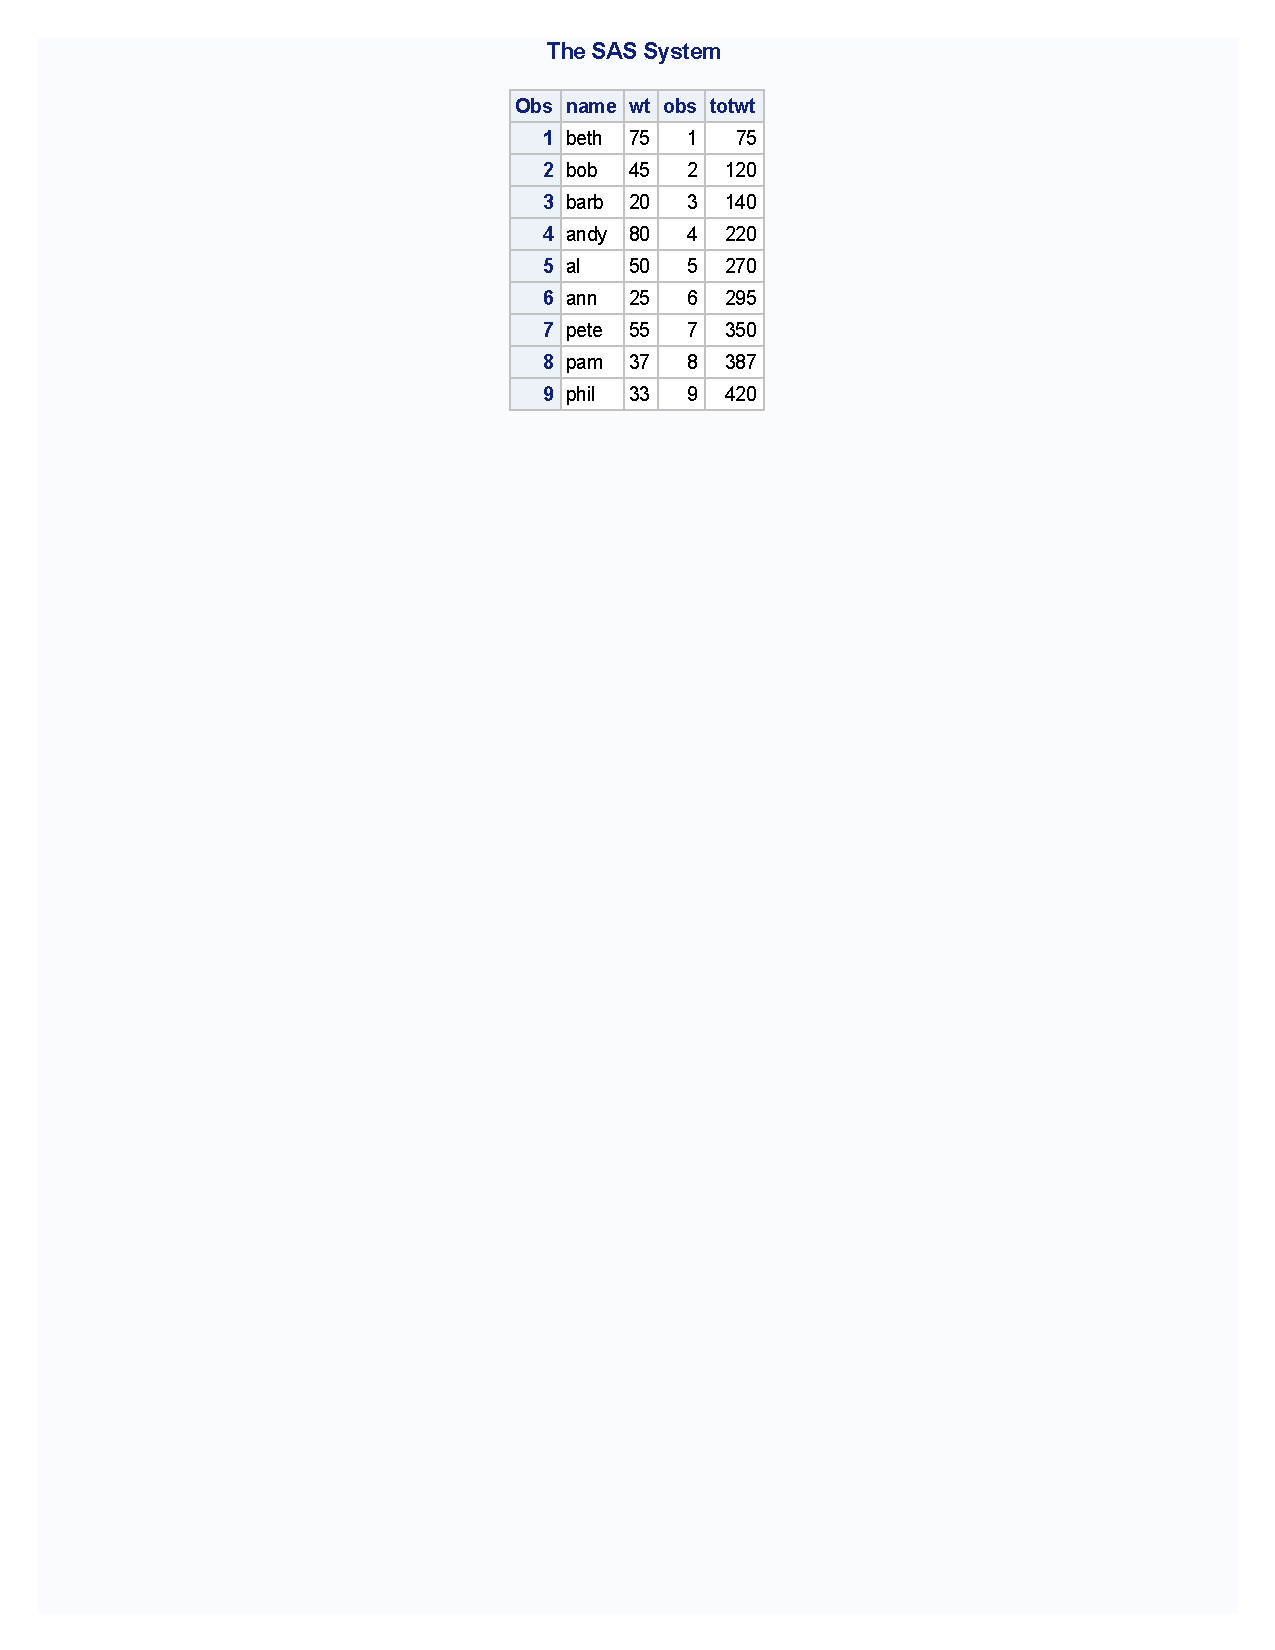
\includegraphics[trim=8cm 21cm 8cm 1.5cm,clip,width=0.7\textwidth]{L14_sum.pdf}
\emp
\end{frame}

\begin{frame}[fragile]
\ft{Example 2 - Cumulative sums}
\bmp{0.65\textwidth}
\footnotesize
\begin{code}{.0}
DATA kids3 ;
   SET kids ;

   obs + 1 ;

   totwt + wt ;

RUN ;
\end{code}
\emp
\bmp{0.05\textwidth} \hspace{0.05in} \emp
\bmp{0.35\textwidth}
\begin{clicker}{What were the initial values of \ttt{obs} and \ttt{totwt}?}
\begin{enumerate}
\item \ttt{.}
\item \ttt{0}
\item \ttt{1}, \ttt{wt}
\item ``  ''
\end{enumerate}
\end{clicker}
\emp
\end{frame}


\begin{frame}[fragile]
\ft{Example 3 - Equivalent sum statements}
\bmp{0.50\textwidth}
\footnotesize
\begin{code}{.0}
DATA kids4;
   SET kids;
   totwt + wt;
RUN;

\end{code}
\bi
\item \ttt{totwt} implicitly initialized to zero
\item use \ttt{SUM} statement \emph{without} variable assignment (no equal sign)
\ei
\emp
\bmp{0.05\textwidth} \hspace{0.05in} \emp
\bmp{0.50\textwidth}
\footnotesize
\begin{code}{.0}
DATA kids5;
   SET kids;
   RETAIN totwt 0;
   totwt = totwt + wt;
RUN;
\end{code}
\bi
\item explicitly initialize \ttt{totwt} to zero
\item use \ttt{SUM} statement \emph{with} variable assignment (equal sign)
\item[]
\ei
\emp
\end{frame}


\begin{frame}[fragile]
\ft{Discussion}
\bmp{0.45\textwidth}
\footnotesize
\begin{code}{.0}
DATA kids3 ;
   SET kids ;

   obs + 1 ;

   totwt + wt ;
   
 
   

RUN ;
\end{code}
\emp
\bmp{0.05\textwidth} \hspace{0.05in} \emp
\bmp{0.5\textwidth}
\oyo How would I modify this code to create a \emph{running average} of weights?  
\emp
%meanwt = sumwt/obs;
\end{frame}

\begin{frame}[fragile]
\ft{Additional \ttt{retain} notes}
\bi
\item the \ttt{RETAIN} statement executes once only when the program compiles
\item so the placement of \ttt{RETAIN} in your data step doesn't matter (the following two sets of statements execute equivalently)
\item[]
\bmp{0.4\textwidth}
\begin{code}{.0}
RETAIN totwt 0 ;  
totwt = totwt + wt ;
\end{code}
\emp
\bmp{0.05\textwidth}\hspace{1in} \emp
\bmp{0.4\textwidth}
\begin{code}{.0}
totwt = totwt + wt ;
RETAIN totwt 0 ;
\end{code}
\emp
\item[]
%\item[]   \fbox{\ttt{RETAIN totwt 0;  totwt = totwt + wt;}}
%\item[]   \fbox{\ttt{totwt = totwt + wt; retain totwt 0; }}
\item \ttt{RETAIN} \ttb{only works with \underline{new} variables}
\item you \underline{cannot} use \ttt{RETAIN} with existing variables
\ei
\end{frame}



%===========================================================================================================================
\section[PROC SORT]{PROC SORT}
%===========================================================================================================================
\subsection{}
\begin{frame}
\tableofcontents[currentsection, hideallsubsections]
\end{frame}


\begin{frame}[fragile]
\ft{PROC SORT syntax}
\bmp{1.0\textwidth}
\footnotesize
\begin{code}{.0}
PROC SORT DATA = \emph{originaldata} OUT = \emph{newdata} ;
    BY \emph{var1} \emph{var2} \emph{var3} ;
RUN ;
\end{code}
\emp
\vskip10pt
\bi
\item the \fbox{\ttt{OUT =}} option is not required
\bi
\item \underline{with:} \emph{newdata} is created (copies \emph{originaldata}) and is sorted
\item \underline{without:} \emph{originaldata} is sorted
\ei
\item \ttt{BY} statement specifies one or more variables to sort by (variables can be either character or numeric)
\bi
\item default sorting order is ascending
\item to reverse, use \ttt{DESCENDING} option \emph{before} the variable name
\ei
\ei
\end{frame}

\begin{frame}[fragile]
\ft{PROC SORT example}
\bmp{0.70\textwidth}
\footnotesize
\begin{code}{.0}
PROC SORT DATA = kids2 OUT = sortedkids ;
   BY DESCENDING famid sex ;
RUN ;
\end{code}
\emp\\
\bmp{0.4\textwidth} \hspace{0.05in} \emp
\bmp{0.6\textwidth}
\begin{craw}{.0}{sortedkids}
Obs famid kidname birth age wt sex
 1    3    pam      2    4  37  f
 2    3    pete     1    6  55  m
 3    3    phil     3    2  33  m
 4    2    ann      3    2  25  f
 5    2    andy     1    8  80  m
 6    2    al       2    6  50  m
 7    1    beth     1    9  75  f
 8    1    barb     3    3  20  f
 9    1    bob      2    6  45  m
\end{craw}
\emp
\end{frame}


\begin{frame}[fragile]
\ft{Discussion}
\bmp{0.65\textwidth}
\footnotesize
\begin{craw}{.0}{output}
Obs famid kidname birth age  wt sex
1     1    barb     3    3   20  f
2     2    ann      3    2   25  f
3     3    pam      2    4   37  f
4     1    beth     1    9   75  f
5     3    phil     3    2   33  m
6     1    bob      2    6   45  m
7     2    al       2    6   50  m
8     2    andy     1    8   80  m
9     3    pete     1    6   55  m
\end{craw}
\emp
\bmp{0.05\textwidth} \hspace{0.05in} \emp
\bmp{0.35\textwidth}
\begin{clicker}{Which BY statement was used in this PROC SORT?}
\begin{enumerate}
\item \ttt{BY obs sex;}
\item \ttt{BY birth sex;}
\item \ttt{BY sex birth;}
\item \ttt{BY DESCENDING birth sex;}
\item \ttt{BY sex DESCENDING birth;} %correct
\end{enumerate}
\end{clicker}
\emp
\end{frame}


%===========================================================================================================================
\section[First./Last.]{First./Last.}
%===========================================================================================================================
\subsection{}
\begin{frame}
\tableofcontents[currentsection, hideallsubsections]
\end{frame}

\begin{frame}
\ft{First./Last. overview}
\bi
\item Recall the automatic variables \ttt{\myuscore N\myuscore } and \ttt{\myuscore ERROR\myuscore }\\
\item Two other automatic variables are \ttt{FIRST.\tte{varname}} and \ttt{LAST.\tte{varname}}\\
	\bi
	\item \ttt{FIRST.\tte{varname}} is an indicator variable (0 or 1) that has a value of 1 when SAS processes the \ttb{first occurrence} of a new value for the variable \ttt{\tte{varname}}\\
	\item \ttt{LAST.\tte{varname}} is an indicator variable (0 or 1) that has a value of 1 when SAS processes the \ttb{last occurrence} of a particular value for the variable \ttt{\tte{varname}}\\
	\ei
\item To access these automatic variables,
\bi
\item use \ttt{PROC SORT} to sort your data \ttt{BY} \emph{varname}
\item in your DATA step, use
\begin{enumerate}
\item \ttt{SET} \emph{sortedata} \ttt{;}
\item \ttt{BY} \emph{varname} \ttt{;}
\end{enumerate}
\ei
\ei
\end{frame}

\begin{frame}[fragile]
\ft{Example 4 - create totals by family}
\bmp{0.55\textwidth}
\footnotesize
\begin{code}{.0}
PROC SORT DATA = kids2 ;
   \textcolor{OrangeRed}{BY famid ;}
RUN ;

DATA kids6 ;
   SET kids2 ;
   \textcolor{OrangeRed}{BY famid ;}

   IF \textcolor{OrangeRed}{FIRST.famid} THEN DO ;
      totwt = 0 ;
      num_kids = 0 ;
   END ;

   totwt + wt ;
   num_kids + 1 ;

RUN ;
\end{code}
\emp
\bmp{0.05\textwidth} \hspace{0.05in} \emp
\bmp{0.40\textwidth} 
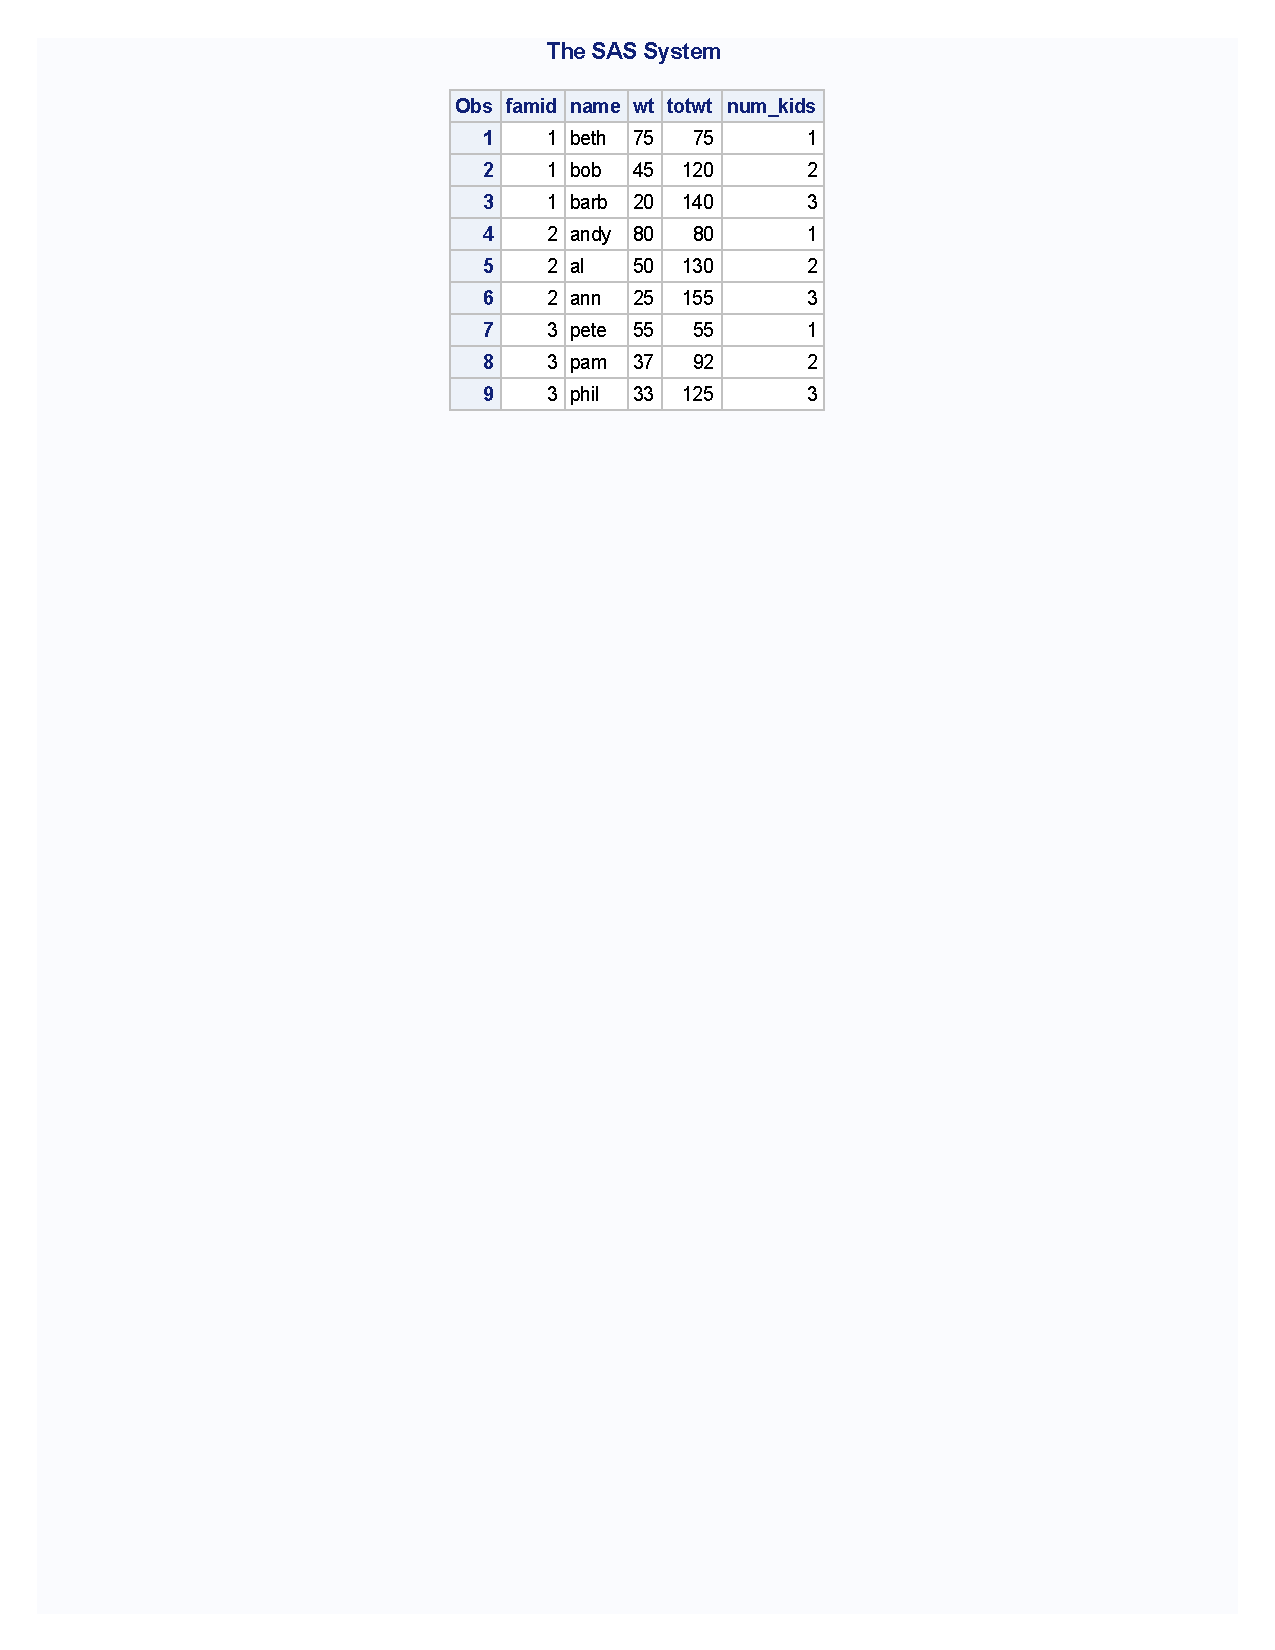
\includegraphics[trim=7cm 21cm 7cm 1.5cm,clip,width=1.0\textwidth]{L14_totalbyfam.pdf}
\emp
\end{frame}



\begin{frame}[fragile]
\ft{Example 4 - create totals by family}
\bmp{0.5\textwidth}
\footnotesize
\begin{code}{.0}
DATA kids6 ;
   SET kids2 ;
   \textcolor{OrangeRed}{BY famid ;}

   IF \textcolor{OrangeRed}{FIRST.famid} THEN DO ;
      totwt = 0 ;
      num_kids = 0 ;
      
      
   END ;

   totwt + wt ;
   num_kids + 1 ;
   
   

RUN ;
\end{code}
\emp
\bmp{0.05\textwidth} \hspace{0.05in} \emp
\bmp{0.40\textwidth}
\oyo 
\begin{enumerate}
\item How could we modify this code to count the number of female and male children per family?
\item How can we view the values of the variable \ttt{FIRST.famid}?
\end{enumerate}
\emp
\end{frame}





\begin{frame}[fragile]
\ft{Example 5 - save family level information}
\bmp{0.55\textwidth}
\footnotesize
\begin{code}{.0}
PROC SORT DATA = kids2 ;
   \textcolor{OrangeRed}{BY famid ;}
RUN ;

DATA kids7 ;
   SET kids2 ;
   \textcolor{OrangeRed}{BY famid ;}
   IF FIRST.famid THEN DO ;
      totwt = 0 ;
      num_kids = 0 ;
   END ;
   totwt + wt ;
   num_kids + 1 ;
   \textcolor{OrangeRed}{IF LAST.famid THEN OUTPUT ;}
   KEEP famid totwt num_kids ;
RUN;
\end{code}
\emp
\bmp{0.05\textwidth} \hspace{0.05in} \emp
\bmp{0.40\textwidth}
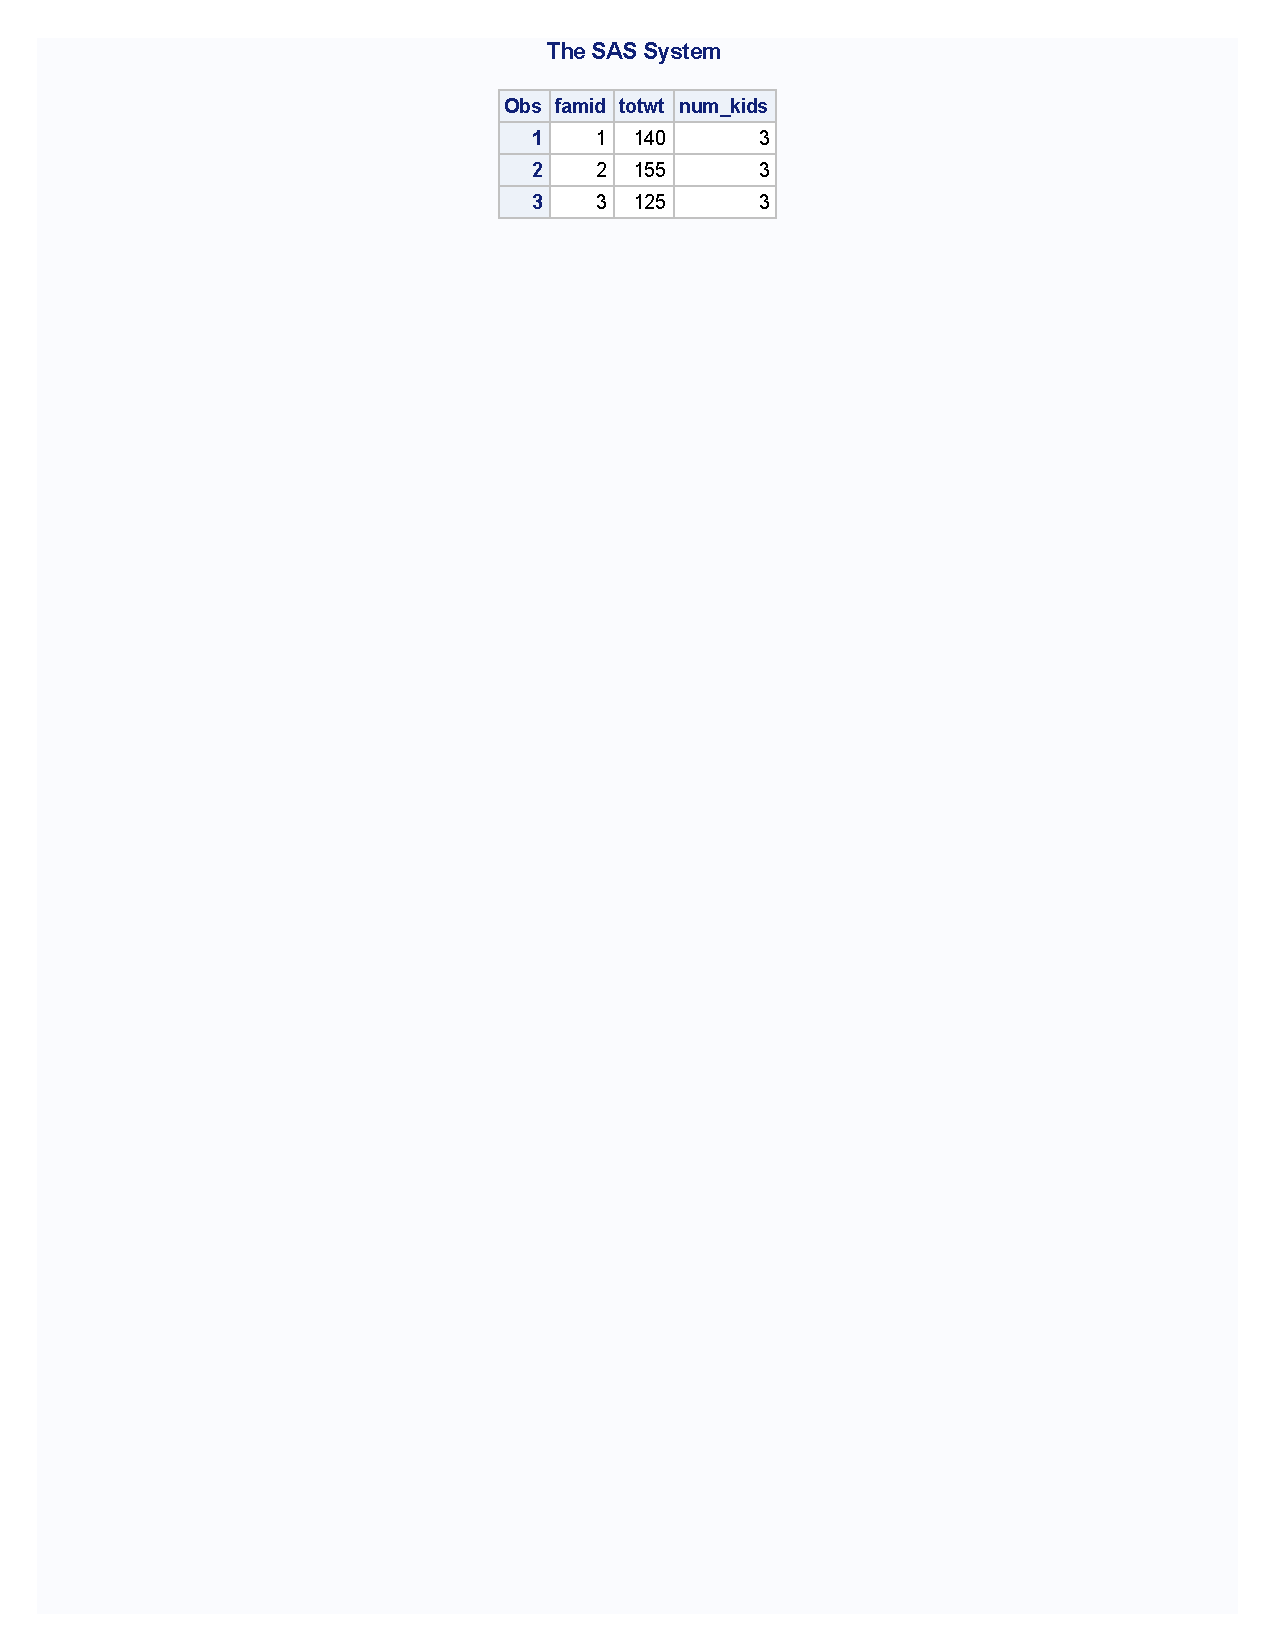
\includegraphics[trim=7cm 21cm 7cm 1.5cm,clip,width=1.0\textwidth]{L14_famtotal.pdf}
\emp
\end{frame}


\end{document} 